\chapter{Intra-node challenges: middleware implementation and evaluation}
As we discussed on the previous chapter, the presented design of our middleware should be able to represent a running system in the form of a model@runtime, according to the Kevoree meta-model.
Indeed, this representation can be manipulated by the existing Kevoree editor, on which we can modify parameters, add or remove nodes and components or bind component's ports using channels.
Therefore, we focus on the intra-node challenges first, by implementing our middleware on real hardware, leveraging our designed platform and existing OS facilities.

In this chapter, we will first explain how the model@runtime can be represented on the IoT device limited memory, as well as the model analysis and manipulation.
%Moreover, means to store a serialized model and easy access to it must be present on the system.
Indeed, as we stated previously, our middleware should also be able to interoperate with the existing Kevoree implementations, in order to achieve interaction with other participants on the internet, such as cloud services, existing distributed applications or simply data mining on remote servers and clients.
Therefore, the standard Kevoree model representation, in the form of a serialized JSON format, is a must-have for our implementation.
This rises several challenges in how a \textit{"big"} (to be saved RAM) representation of the model can be stored and accessed on our constrained nodes.
We will present how we cope with this challenge, from the representation of objects in a procedural language such as C, to the manipulation techniques used to compare and execute the actions described on the models.

Experiments were conducted to evaluate the functionalities and the scalability of our approach, and the results are presented at the end of the chapter.
First, a generic implementation is tested on a single \textit{"big"} node, followed by scalability experiments on a typical node present in a large-scale testbed.
Our main goal is to state the minimal functionalities at the model level, from which we can then implement the needed mechanisms to achieve real reconfigurations and adaptations described in the new upcoming models.

%However, in order to realize these modifications, system facilities should be leveraged, such as component instantiation, deploy unit downloading, and dynamic loading of binaries for new deployments.
%In this chapter, we discuss the current requirements from the underlying system, as well as the hardware device features (\textit{i.e.} connectivity, storage) needed to achieve a dynamic behavior.
%Afterwards, some technical contributions to an IoT operating system will be presented, since the complexity of our middleware leads to specific OS requirements that are not often provided.
\section{An empirical study on constrained IoT devices}
The model@runtime paradigm has been mainly investigated in the context of distributed systems. 
These research efforts have been focused on the provision of a comprehensive set of tools to easily deploy, dynamically reconfigure, and disseminate software on a set of distributed computing units.
The current model@runtime tools have been implemented regardless of the specific characteristics and constraints of IoT devices.
In particular, the network topology and the resource constraints of the nodes forming the distributed system have not been taken into consideration.
As a result, state of the art model@runtime tools are not suitable to be used in the context of IoT Systems.
%First, most approaches are relying on the Java language, which does not meet the resource constraints of the computing nodes. 
%Secondly, the size of the model and its distribution among the system are not taking into consideration the limited memory capacity of each node, and their energy constraints.

In  \cite{fouquet2012dynamic} $\mu$-Kevoree, the closest effort to port the model@runtime paradigm on the constraints of a Cyber Physical System (CPS) was presented, in which the underlying device is comparable to an IoT device.
Despite the particular attention given to the specific constraints of a Cyber Physical System, this work heavily relies on over the air firmware flashing to support the deployment and reconfiguration of software. 
We consider that relying on firmware flashing to support software deployment constitutes a flaw in the approach because of its energy cost (the complete firmware has to be sent, and if any error occurs, the whole process is restarted).
A second limitation of this approach lies in the fact that each resource constrained node relies on a more powerful node to perform most of its tasks related to the dynamic reconfiguration (firmware synthesis, reconfiguration decision and so on).
This second limitation is not suitable in the context of a system mainly composed by resource constrained nodes since all these nodes have to be managed by bigger nodes.
Pushing this idea further, the management of a CPS composed of a wide number of resource constrained devices and a bigger node, the latter will have to manage all the smaller devices in a centralized management scheme.

The next section will describe a more complete M@R engine implementation based on the Kevoree meta-model, together with some tools which allow model manipulation.

\subsection{Kevoree-IoT: Estimating needed resources}
\label{subsec:MARImpl}
%Since our work aims to provide a M@R engine for IoT devices, a first implementation should be developed having in mind the programming constraints.
%Taking into account this limitations means that, first of all, we must fit the programming constraints.
In contrast with most of the current implementations of the M@R paradigm, which are intended for high resources machines thus they make use of high-level programming languages, our first implementation should follow a procedural language such as C.
We can justify this by the fact that most of the open source compilers for IoT devices support only this programming language, in addition to C++.
However, C++ applications are difficult to integrate in OSs like Contiki or RIOT, which are convenient OS able to run our middleware.
Thus, a first approach has been developed in plain C\footnote{\url{https://github.com/kYc0o/kevoree-c}} following the directions presented in Section \ref{sec:kevAndIoT}.
%This raised big challenges since the object-oriented meta-model representation is very difficult to transform into C structures, knowing that there is no modelling framework supporting such a language.

%\begin{table}[]
%	\centering
%	\caption{Size of a plain C minimalistic Kevoree meta-model implmentation}
%	\label{tab:kevoreeC}
%	\begin{tabular}{|c|c|c|c|}
%		\hline
%		\textbf{text (ROM)}   & \textbf{data (RAM)} & \textbf{bss (zeroed RAM)} & \textbf{overall size} \\ \hline
%		181997 & 1448 & 168 & 183613 \\ \hline
%	\end{tabular}
%\end{table}

\begin{figure}[]
	\centering
	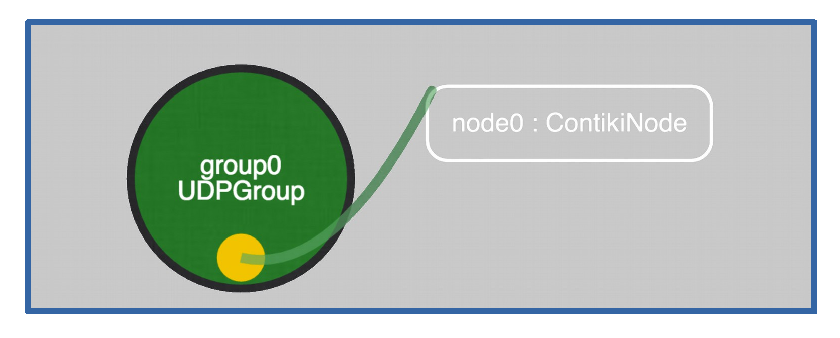
\includegraphics[width=0.55\columnwidth]{chapters/intra-node.images/MAR_example.pdf}
	\caption{Graphical representation of a minimal M@R}
	\label{fig:1stModelC}
\end{figure}

Indeed, our efforts were put into a first manual implementation of the Kevoree meta-model.
The size of the test application which contains a group and a node without components is of 181997 bytes, while the needed RAM before the execution is of 1616 bytes. % shown in table \ref{tab:kevoreeC}
A graphical representation of the model can be obtained through the Kevoree Web Editor\footnote{\url{http://editor.kevoree.org/v4/}}, in which a serialized JSON file containing the model can be loaded for edition.
This representation is shown in figure \ref{fig:1stModelC}.

%Our firsts results show that approximately 180KB of ROM space (text) are needed for the implementation, while 14KB of RAM (data + bss) were enough for such application.
%This test was compiled using the GCC (GNU C Compiler) version 4.9, for a i386 32-bit platform.
%Therefore, we need to find an IoT device which fit this minimal requirements.

Then, it is necessary to characterize the minimum system requirements for an IoT device to implement a full model@runtime middleware, as in hardware capabilities as in execution environment.
This will avoid the use of third party nodes to perform the high level tasks described above.
However, even if a proposed device meet the characteristics to perform such tasks, the trade-offs between energy consumption and the middleware execution should be taken into account.
A general description of needed features to execute the proposed middleware is given in the next subsection.

%\subsection{Needed features of the underlying system}
\subsection{Handling hardware constraints}
%Currently the concept of model@runtime has been applied on top of object oriented languages which offers the required features at the language level to implement the model@runtime layer. 
%The first challenge lies in the fact that Contiki does not support these object oriented languages and thus the design must fit a procedural language such as C.

%The second challenge lies in the very limited resources of the IoT nodes, thus forcing the middleware to meet the memory and CPU constraints. 
%This imposes constraints on the way the model is represented, stored and processed on each node.
%This challenge is particularly important and hard to meet, since many software components are needed to enable the communication in these environments (radio/MAC/IP stack and so on).
Considering the challenges presented in Section \ref{sec:kevAndIoT}, we must test our implementation on real hardware platforms in order to measure the limitation of our approach, as well as its compatibility with the other implementations (Java, Cloud, Android).
Moreover, the energy constraint of each IoT node, together with the mesh topology of the network makes communication in this environments fairly reliable.
This implies the necessity to optimize the way the model and the software are disseminated on the network.

At first glance, our implementation was compiled for three different platforms (\textit{class 1 \cite{rfc7228}}): the \textit{\textbf{zolertia Z1\footnote{\url{http://zolertia.sourceforge.net/wiki/images/e/e8/Z1_RevC_Datasheet.pdf}}, redbee econotag\footnote{\url{http://redwire.myshopify.com/products/econotag-ii}} and wismote\footnote{\url{http://wismote.org/doku.php}}}}, which were widely used for research purposes in the IoT domain.
Unfortunately, none of these platforms was able to meet the space requirements in ROM and RAM to run a minimal model at runtime as shown in figure \ref{fig:1stModelC}.
However, the existence of more powerful microcontrollers, an essential part of an IoT device, shows that typical IoT applications have not exceeded the resources of existing experimentation platforms.
Indeed, only some development kits such as TI's CC2538DK\footnote{\url{http://www.ti.com/tool/cc2538dk}} were available at that time, but its high cost, low availability and poor support gave low acceptance for research purposes.
Thus, the design and construction of a new experimentation platform seemed to be the fastest way to obtain the first results of the implementation, by integrating the latest microcontrollers and peripherals available on the market.
It is worth to consider that this platform was conceived for research and experimentation purposes, and not as an end-user device.

An exhaustive search was conducted to find the latest technologies to build an experimentation IoT device, which fits the requirements already estimated in section \ref{subsec:MARImpl}.
The first step was to find the basic components of such a device.
Taking into account the requirements from section \ref{sec:kevoreeRequirements}, an IoT device should, more specifically, embed:
\begin{enumerate}
	\item \textbf{Microcontroller.} A low-power microcontroller unit is needed to perform the computational processing tasks as well as to store the program code. 
	A huge amount of ROM and RAM is needed at the scale of these devices, thus it is necessary to find a microcontroller with a good trade-off between energy consumption and memory size.
	\item \textbf{Communication interface.} Communication is the main task that will perform our device, since it is mandatory for IoT environments.
	A radio interface implementing the widely used IEEE 802.1.5.4 standard \cite{ieee802.15.4} is then necessary to communicate in an interoperable way with other devices.
	An ultra-low energy consumption is also important, since communication is the most energy consuming task.
	\item \textbf{External flash memory.} Storage for data is a very useful feature for an IoT device. It can serve as persistent data storage for logging and data collection from sensors, as well as updates and eventually new firmwares.
	\item \textbf{Sensors and actuators.} In order to collect experimentation data, some sensors should be embedded on the device, the most common being temperature, humidity and position.
	Indicator LEDs are also commonly present in these devices, to provide visual signs such as function status (ON/OFF) or current communication.
	\item \textbf{Ports for external devices.} An easy way to connect third party devices allows a dynamic behaviour, since we can connect other sensors, actuators and devices which cannot be present internally on the device.
	Such devices should be connected using standard interfaces, such as I2C and SPI.
	General Purpose Inputs/Outputs (GPIO) are also widely used, either as digital or analog interfaces.
	\item \textbf{Battery capabilities.} An IoT device is very often used in environments where a constant power source is not present.
	Thus, work on batteries is a very useful feature to test energy consumption while adding flexibility of placement.
\end{enumerate}

Given these features, it was then necessary to integrate several components in order to build the required IoT device.
We put special attention to the most critical components, which are the microcontroller, the external flash memory and the battery controller.
Regarding the radio transceiver and the other peripherals, there are no huge differences between the most commonly used, for instance, the ones used in the previously analysed devices.
The specific conception of the platform will be described in the next subsection.

\subsection{Towards a new IoT device}
\label{subsec:newIoTDevice}
Several low-power microcontroller architectures were available at the time of our first M@R implementation, such as TI MSP430, Atmel AVR, Microchip PIC and ARM Cortex-M, just to mention the most common ones.
Since our middleware minimum memory requirements were tested on 16-bit MSP430 microcontrollers (Zolertia's Z1 and Arago's WiseMote), finding a huge scarcity of memory, 32-bit architectures were the target of our scope.
Indeed, ARM Cortex-M microcontrollers offer only 32-bit RISC architectures, which are widely used both in research and industry.
Thus, the first step was to select an ARM Cortex-M microcontroller fitting our memory and energy consumption requirements.
The ST Microelectronics STM32 family of microcontrollers offers a wide range of devices with different processor speeds and memory sizes.
%\begin{figure}[]
%	\centering
%	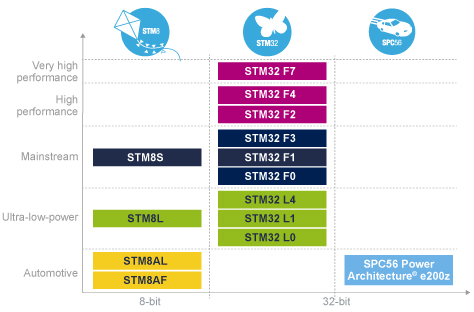
\includegraphics[width=0.70\columnwidth]{chapters/intra-node.images/STM32.jpg}
%	\caption{STM32 Microcontroller family}
%	\label{fig:STM32}
%\end{figure}
%Figure \ref{fig:STM32} shows the STM32 family applications and available solutions for each one.

%At the time of this search, ultra-low-power solutions (STM32L) were not available, thus our possibilities were in the STM32F range, excluding the F7 which was also released recently.

\begin{table}[]
	\centering
	\caption{Comparison between STM32F microcontrollers}
	\label{tab:STM32F}
	\begin{tabular}{c|cccc}
		Microcontroller & Speed (MHz) & RAM (KB) & ROM (KB) & \begin{tabular}[c]{@{}c@{}}Consumption \\ at max. speed (mA)\end{tabular} \\ \hline
		STM32F0         & 48          & 32       & 256      & 22                                                                        \\
		STM32F1         & 72          & 96       & 1024     & 68                                                                        \\
		STM32F3         & 72          & 80       & 512      & 61.5                                                                      \\
		STM32F2         & 120         & 128      & 1024     & 49                                                                        \\
		STM32F4         & 180         & 256      & 2048     & 98                                                                       
	\end{tabular}
\end{table}

Since our goal is to build a device on which our experimentations could be executed on a more flexible way (without caring about memory requirements), it is preferable to use a microcontroller featuring the highest memory capabilities, both in ROM and RAM, over energy consumption.
Moreover, these kind of devices are able to change the processor speed as needed, thus reducing the energy consumption.
Indeed, our choice was a STM32F4 microcontroller, which was used as the core of our IoT device.
Table \ref{tab:STM32F} shows a comparison between the available microcontrollers, featuring the maximum processor speed, RAM and ROM, followed by the current consumption in such configuration.

As for the power scheme, given the capabilities of the selected microcontroller, a power source between 1.8V and 3.6V is required.
Indeed, a first approach to power the device is the use of an USB port, which delivers around 5V.
Thus, a 5V to 3.3V (the recommended tension) is required.
In contrast, when the device is needed to run on batteries, the supplied voltage will change.
%The most common batteries available on the market provide between 1.5V (AA, AAA) and 3V (CR3032), which is in the acceptable range.
A couple of AA batteries connected in series is the most standard array to power IoT devices.
However, a wide set of peripherals such as sensors and actuators work very often at 5V.
Therefore, it was necessary to add a DC to DC converter, coupled with an automatic power selector which detects when the device is powered either by USB or batteries.
This allows to use any power scheme without decreasing performance or peripherals compatibility.

\begin{table}[]
	\scriptsize
	\centering
	\caption{IoT Platforms comparison}
	\label{tab:IoTPlatfComp}
	\begin{tabular}{cccccccc}
		\textbf{}                                                                               & \textbf{\begin{tabular}[c]{@{}c@{}}Speed \\ (MHz)\end{tabular}} & \textbf{\begin{tabular}[c]{@{}c@{}}RAM \\ (KB)\end{tabular}} & \textbf{\begin{tabular}[c]{@{}c@{}}ROM \\ (KB)\end{tabular}}                               & \textbf{\begin{tabular}[c]{@{}c@{}}External \\ flash (MB)\end{tabular}} & \textbf{\begin{tabular}[c]{@{}c@{}}Radio \\ transceiver\end{tabular}} & \textbf{Peripherals}                                                                                    & \textbf{\begin{tabular}[c]{@{}c@{}}Embedded\\ Sensors\end{tabular}}                                \\ \cline{2-8} 
		\multicolumn{1}{c|}{\textbf{\begin{tabular}[c]{@{}c@{}}Zolertia \\ Z1\end{tabular}}}    & \multicolumn{1}{c|}{16}                                         & \multicolumn{1}{c|}{8}                                       & \multicolumn{1}{c|}{96}                                                                    & \multicolumn{1}{c|}{2}                                                  & \multicolumn{1}{c|}{CC2420}                                           & \multicolumn{1}{c|}{\begin{tabular}[c]{@{}c@{}}UART, I2C\\ Phidgets \\ (USB only),\\ GPIO\end{tabular}} & \multicolumn{1}{c|}{\begin{tabular}[c]{@{}c@{}}3 axis acc.\\ and\\ temperature\end{tabular}}       \\ \cline{2-8} 
		\multicolumn{1}{c|}{\textbf{\begin{tabular}[c]{@{}c@{}}Arago's\\ WisMote\end{tabular}}} & \multicolumn{1}{c|}{25}                                         & \multicolumn{1}{c|}{16}                                      & \multicolumn{1}{c|}{256}                                                                   & \multicolumn{1}{c|}{8}                                                  & \multicolumn{1}{c|}{CC2520}                                           & \multicolumn{1}{c|}{\begin{tabular}[c]{@{}c@{}}UART, I2C,\\ Phidgets, \\ GPIO\end{tabular}}             & \multicolumn{1}{c|}{\begin{tabular}[c]{@{}c@{}}3 axis acc.\\ light and\\ temperature\end{tabular}} \\ \cline{2-8} 
		\multicolumn{1}{c|}{\textbf{\begin{tabular}[c]{@{}c@{}}Redbee\\ econotag\end{tabular}}} & \multicolumn{1}{c|}{26}                                         & \multicolumn{1}{c|}{96}                                      & \multicolumn{1}{c|}{\begin{tabular}[c]{@{}c@{}}N/A\\ (device run\\ from RAM)\end{tabular}} & \multicolumn{1}{c|}{128 (KB)}                                           & \multicolumn{1}{c|}{Integrated (SoC)}                                 & \multicolumn{1}{c|}{GPIO}                                                                               & \multicolumn{1}{c|}{N/A}                                                                           \\ \cline{2-8} 
		\multicolumn{1}{c|}{\textbf{\begin{tabular}[c]{@{}c@{}}DiverSE\\ Board\end{tabular}}}   & \multicolumn{1}{c|}{180}                                        & \multicolumn{1}{c|}{256}                                     & \multicolumn{1}{c|}{2048}                                                                  & \multicolumn{1}{c|}{16}                                                 & \multicolumn{1}{c|}{CC2520}                                           & \multicolumn{1}{c|}{\begin{tabular}[c]{@{}c@{}}UART (x2), \\ I2C\\ Phidgets, \\ GPIO\end{tabular}}      & \multicolumn{1}{c|}{N/A}                                                                           \\ \cline{2-8} 
	\end{tabular}
\end{table}

\begin{figure}[htb]
	\centering
	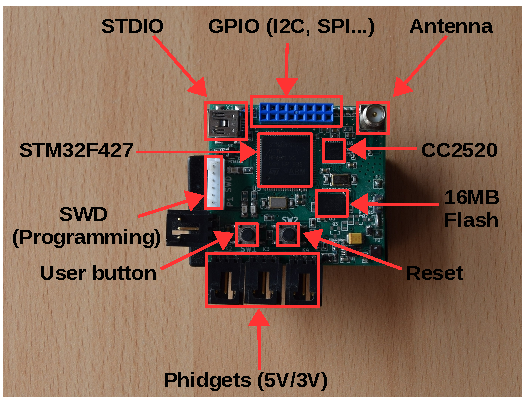
\includegraphics[width=0.7\columnwidth]{chapters/intra-node.images/newBoard.pdf}
	\caption{The new designed board to meet our needs.} \label{fig:newBoard}
\end{figure}

Thus far, the main required features for our device are met.
A comparison between the previously tested platforms and ours is given in table \ref{tab:IoTPlatfComp}, showing the most common useful features.
Moreover, figure \ref{fig:newBoard} shows the layout of the new board, on which we can observe the different components and the size of the PCB.
Indeed, its measures are 3.5cm x 4.5cm.
%Details about the other components such as the radio transceiver and the external flash memory can be found in \todo{annex X.}

Given the features of our new IoT device, the next step is to provide the hardware abstraction layer and a network stack to integrate it into an IoT network.
Indeed, several IoT operating systems existed at the time this device was developed, thus leveraging one of these available OS was the most recommended procedure.
%The next Subsection discuss the implementation of all the necessary tools to integrate our middleware into this new platform, making the choice of porting the Contiki OS to support our IoT device.
It is important to notice that our middleware implementation it's independent of the underlying OS, since it only provides abstractions for the representation of the running system in the form of a model@runtime.
Thus, it can be adapted to any other OS able to integrate modules written on C, as well as networking facilities typical of the IoT to disseminate such model.


\section{The new Kevoree-IoT Contiki implementation}
\label{subsec:kevoreeContikiImpl}
In this section, we present our initial results towards the design of a middleware which will offer the functionalities of model@runtime over the previously conceived IoT device. 
%Porting the concept of model@runtime on IoT devices will enable a continuous management of the deployed software.
This middleware, which we called Kevoree-IoT (in reference to the kevoree-like M@R implementation of our middleware), will provide a development framework for applications on top of these systems, and will provide the runtime infrastructure to support the deployment and dynamic reconfiguration of these applications.

We based our implementation on an already ported Contiki version\footnote{\url{https://github.com/vedderb/contiki}} for a very similar device than ours, which provided a basic hardware abstraction layer for the radio interface and some I/O drivers.
The rest of the drivers were developed according to our platform hardware design.
Once the porting completed the next step was to test our middleware on such platform.
To do that, a Kevoree-IoT application should be developed, using this new Contiki port.


%As illustrated in figure \ref{fig:ContributionOverview}, our goal is to provide a middleware that will be present on each node of the system, and will take care of the various tasks imposed by the model@runtime paradigm.
%More specifically, our middleware will be in charge of:
%\begin{enumerate}
%	\item Receiving new models that define the new targeted state of the system,
%	\item Defining the set of local adaptations that are needed to reach this new state,
%	\item Enacting the various local adaptations produced by the previous step.
%\end{enumerate} 

%The set of local adaptations enables the dynamic reconfiguration and may download new software artifacts, instantiate or remove components and channels used to bind them, or reconfigure the value of any attribute.

Based on the Kevoree-C implementation introduced in subsection \ref{subsec:MARImpl}, the needed Contiki application was developed and tested in our platform.
The first implementation\footnote{\url{https://github.com/kYc0o/kevoree-contiki}} was done using the version 4 of the Kevoree meta-model.
This meta-model has been mapped into C code as a Contiki application.
We were able to add nodes, components, groups and channels, and bind them through the Kevoree editor by loading a generated JSON file.

\subsection{An object-oriented representation using C}
As we discussed previously on Subsection \ref{subsec:minKevProp}, special attention must be put while transforming a meta-model into a procedural language such C.
Indeed, this programming language does not have an object-oriented design, thus a representation of classes, their properties and relationships from the Kevoree meta-model should be proposed.

We took as a source of inspiration the existing Kevoree implementation for C++\footnote{\url{https://github.com/kevoree/kevoree-cpp}}, which is the closest language that match with C.
In this implementation, the classes and its relationships are transformed into C++ code directly, since it supports object-oriented representations.
We can observe four components in the Kevoree meta-model:

\begin{itemize}
	\item \textbf{Classes.} This is the abstract representation of an object type. It can be instantiated and contains properties and relationships with other classes.
	\item \textbf{Properties.} Values that can have the form of a primitive type (integer, character, boolean, etc.), depending on the types supported by the language. Special properties called methods are also part of a class, which provide a specific functionality when the method is called.
	\item \textbf{Relationships.} These are the connections between two or more classes. We can note two types: a reference and a containment reference.
	\item \textbf{Inheritance.} A class can inherit the previously described components from another one, besides adding its own.
\end{itemize}

Thus, implementing this representation lead our efforts to optimize the resulting code, while respecting the previously described composition.
Indeed, the first step was to represent a class as a C data structure.
While doing it, some decisions were made in order to cope with the intra-node constraints:

\begin{itemize}
	\item Primitive types such as integers and boolean keep the same size as in the meta-model.
	\item String types are of a fixed size, to avoid dynamic memory allocation thus eventual fragmentation.
	\item Methods are represented as function pointers, in a separated structure called \textit{Virtual Table}, allowing easy inheritance.
	\item Properties inheritance is achieved by copying the parent's properties (including and respecting all the inheritance hierarchy), followed by a pointer to the virtual table. This way we can reuse code and ensure polymorphism.
	\item References are represented as a pointer to the referenced structure, while containment is achieved using a minimalistic implementation of a hashmap.
\end{itemize}

\lstset{language=C,
	basicstyle=\ttfamily\scriptsize,
	keywordstyle=\color{blue}\ttfamily,
	stringstyle=\color{red}\ttfamily,
	commentstyle=\color{gray}\ttfamily,
	breaklines=true,
	captionpos=b
}

\begin{lstlisting}[language=C, caption=KMFContainer: the main container on Kevoree, label=lst:KMFContainer]
typedef char* (*fptrKMFMetaClassName)(void*);
typedef char* (*fptrKMFInternalGetKey)(void*);
typedef char* (*fptrKMFGetPath)(void*);
typedef void (*fptrVisit)(void*, char*, fptrVisitAction, fptrVisitActionRef, bool);
typedef void* (*fptrFindByPath)(void*, char*);
typedef void (*fptrDelete)(void*);

typedef struct _KMFContainer_VT {
void *super;
/*
* KMFContainer_VT
*/
fptrKMFMetaClassName metaClassName;
fptrKMFInternalGetKey internalGetKey;
fptrKMFGetPath getPath;
fptrVisit visit;
fptrFindByPath findByPath;
fptrDelete delete;
} KMFContainer_VT;

typedef struct _KMFContainer {
    KMFContainer_VT *VT;
    /*
    * KMFContainer
    */
    KMFContainer *eContainer;
} KMFContainer;
\end{lstlisting}

\begin{lstlisting}[language=C, caption=NamedElement class representation inheriting from KMFContainer, label=lst:NamedElement]
typedef struct _NamedElement_VT {
    KMFContainer_VT *super;
    /*
    * KMFContainer
    * NamedElement
    */
    fptrKMFMetaClassName metaClassName;
    fptrKMFInternalGetKey internalGetKey;
    fptrKMFGetPath getPath;
    fptrVisit visit;
    fptrFindByPath findByPath;
    fptrDelete delete;
} NamedElement_VT;

typedef struct _NamedElement {
    NamedElement_VT *VT;
    /*
    * KMFContainer
    */
    KMFContainer *eContainer;
    /*
    * NamedElement
    */
    char name[16];
} NamedElement;
\end{lstlisting}

We can observe on listing \ref{lst:KMFContainer} the representation of the main Kevoree class \textit{KMFContainer} which includes only a pointer to its container and a pointer to the Virtual Table containing the function pointers to its methods.
As an example, the class \textit{NamedElement} in listing \ref{lst:NamedElement} shows how inheritance is achieved, by copying the property of the parent class.
On the other hand, method inheritance is achieved by copying all the function pointers into its own virtual table. 
Moreover, to access parent's method implementation, the virtual table contains also a pointer to its parent (super class).

Once a representation of the basic requirements is implemented, we need to provide mechanisms to represent an instantiated model using the data structures described previously.
The next Subsection describes briefly how the process of serialization and de-serialization takes place.

\subsection{Model manipulation challenges}
While representing an instantiated model in memory, we need to allocate enough place for the required nodes, components and connections that are described in a serialized form.
This starts by a model de-serialization, which consists in the transfer of a JSON file among the nodes in the network, followed by the model parsing and execution of the adaptations and reconfigurations described on it.
Due to memory limitations, a model cannot be loaded entirely, thus mechanisms to partial loading and parsing should be provided.
Indeed, a very efficient JSON loader was developed to fit the memory constraints.
This loader takes the JSON elements one by one directly from the external flash, thus avoiding the allocation of big memory slots, and freeing the already parsed elements.
Once an element is loaded, it is compared with the current status of the system (the running model being de-serialized at the same time), generating a list of differences (traces about changes) which are analysed to create a list of adaptations and reconfigurations.

The execution of the adaptations and reconfigurations will leverage the features provided by the underlying system, which were already presented in section \ref{sec:kevoreeRequirements}.

\section{Firsts evaluations of the approach}
Our firsts results showed that our implementation was able to run on our experimentation device.
This first firmware contains the Contiki OS kernel, device drivers, a CoAP web server and the Kevoree-IoT middleware.
The memory size of this firmware is of 215228 bytes in ROM and only 18404 bytes in RAM.% shown in table \ref{tab:kevoreeContiki}.

%\begin{table}[htb]
%	\centering
%	\caption{Size of a minimalistic Contiki application usign Kevoree-IoT}
%	\label{tab:kevoreeContiki}
%	\begin{tabular}{|c|c|c|c|}
%		\hline
%		\textbf{text (ROM)}   & \textbf{data (RAM)} & \textbf{bss (zeroed RAM)} & \textbf{overall size} \\ \hline
%		215228 & 3508 & 14896 & 233632 \\ \hline     
%	\end{tabular}
%\end{table}


Once our middleware was running in our experimental platform, we needed to test it at large scale in order to test the model dissemination.
This needs a large infrastructure with several devices where a basic experiment using our middleware can be executed.
Indeed, the manufacturing of several of our devices was our first option.
However, since the manufacturing of the firsts devices was made by hand, to build some other a huge amount of time was needed, and could be very costly.
Therefore, a search for large-scale testbeds for the IoT was done.
The next section will describe one of the platforms available in a large-scale testbed, showing its main characteristics, which were analysed in order to find if they met our requirements.

\subsection{Requirements for large-scale evaluation}
\label{sec:iotlab}
At the time of our firsts experiments, a testbed existed at the INRIA Rennes centre, where our research team is based.
A Wireless Sensor Network called Senslab \cite{des2011senslab}, formed by 256 devices was deployed in a centre's cellar.
This WSN offered wireless sensors of similar characteristics as the Z1 platform, which was already described.
Thus, the minimum requirements to run our middleware were not met by these WSN's devices.
However, an extension of such testbed was done recently, adding new experimentation platforms.
This new platform, called FIT IoT-Lab \cite{Fleury15iotlab}, featured new devices of a similar architecture as ours.
Indeed, two more powerful nodes were added to the testbed: the M3 node and the A8 node, in order to provide more powerful IoT capabilities.

\begin{figure}[htb]
	\centering
	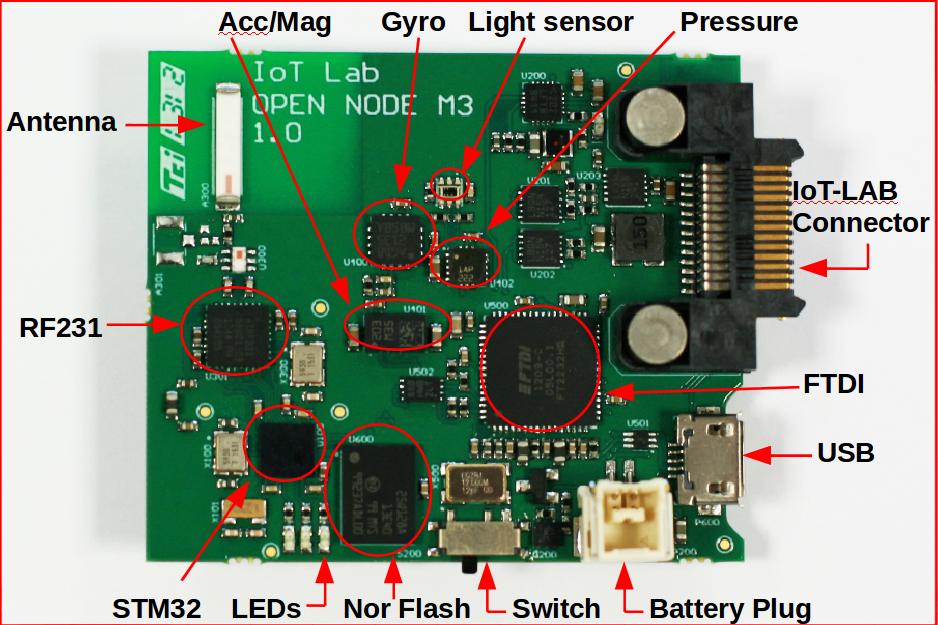
\includegraphics[width=0.7\columnwidth]{chapters/intra-node.images/m3opennode.png}
	\caption{The FIT-IoT Lab M3 Open Node} \label{fig:M3OpenNode}
\end{figure}

Figure \ref{fig:M3OpenNode} presents the M3 Open Node, an IoT device with very similar characteristics of the one from our design.
This device features a STM32F1 Cortex-M3 microcontroller, with 512KB of ROM and 64KB of RAM.
External sensors are available, as well as 3 LEDs.
The communication is handled by an AT86RF231 radio, implementing the standard IEEE 802.15.4, typical of IoT devices.
In addition, a Contiki port for this device was already available, facilitating the integration of our existing implementation for Contiki.
This combination seems suitable for our experiments, since our firsts results showed that around 200KB of ROM and 16KB of RAM were enough to run a minimal implementation of our middleware, including the kernel, communication stack and peripheral drivers.

The next subsection will give details about the technical contributions provided for the IoT-Lab testbed, in order to have a complete IoT platform able to run our middleware and ready for our large-scale tests.
Indeed, testing on a large scale testbed facilitates the firmware flashing, serial output for debugging and power monitoring, thanks to the tools provided by IoT-Lab\footnote{\url{https://www.iot-lab.info/tools/}}.
Moreover, a Contiki port is maintained and supported by the IoT-Lab team, providing a ready to use environment for our already developed tools.
% as we already introduced on section \ref{sec:iotlab}
However, two important features lacked in this port: the low-level interface for the Contiki File System (CFS) and the relocation operations needed by the Contiki ELF loader.
Therefore, given the importance of these features for the correct implementation of our middleware, it was necessary to extend the testbed capabilities to add support for the CFS and the ELF loader.


\subsection{Extending the FIT IoT-Lab testbed}
As stated previously, two missing features were detected in the Contiki port made for this testbed.
The first one was the implementation of a low-level interface necessary for the Contiki File System.
This driver make use of low-level functions to read, write and erase the flash memory embedded on the M3 node.
Therefore, this functionality is necessary to leverage the high-level abstractions provided by the CFS, which are a very useful approach to manipulate files into the flash memory, also needed by the ELF loader.

%\todo{Until here it's ok, the rest of the chapter needs to be reworked}

\subsubsection{File system driver implementation}
The definitions and porting instructions for CFS can be found on the wiki page of the Contiki main repository\footnote{\url{https://github.com/contiki-os/contiki.git}} as well as in the article introducing this file system in  \cite{tsiftes09enabling}.
A brief description of the file system is given as follows:

\begin{citeverbatim}
	Contiki provides a set of file systems for using various kinds of storage devices in resource-constrained systems. 
	All of these file systems implement a subset of the Contiki File System (CFS) interface, and two of them provide the full functionality: CFS-POSIX and Coffee.
	CFS-POSIX is used in Contiki platforms that run in native mode. 
	It uses direct calls to the POSIX file API that is provided by the host operating system. 
	Coffee, on the other hand, is primarily aimed at sensor devices that are equipped with flash memories or EEPROM.
\end{citeverbatim}

Thus, the usage of the \textit{Coffee} API is the one that should be implemented for the M3 platform.
To do so, information about the flash memory embedded on the platform must be mapped into the configuration headers used by Contiki, in order to provide a connection between the physical device and the OS.
This information consists in several parameters, such as:
\begin{description}
	\item[Total size.] The actual size of the memory flash.
	\item[Sector size.] A flash memory is divided by sectors. This information allows the CFS to organize the way the memory will be written.
	\item[Page size.] This parameter is given by the manufacturer of the flash memory and allows to organize writing cycles in a more efficient manner, avoiding fragmentation.
	\item[Coffee start.] It describes the actual memory address where Coffee can start to write. It allows to reserve a memory space that cannot be accessible from the API, providing a secure space where we can store read-only data (\textit{i.e.} initialization data, node ID, etc.).
	\item[Coffee size.] This is the overall memory available for reading/writing using Coffee. It is calculated by the difference between the total size and the Coffee start size.
	\item[Coffee name length.] With a view on internal memory savings, a limitation on file names is imposed. This will avoid the use of large filenames which have an impact on the memory footprint of the CFS.
	\item[Coffee max. open files] In the same way as name length, the number of simultaneous open files can increase the memory usage by the file system. Thus, a limitation on this concern is needed.
\end{description}

Afterwards, parameters to configure the internal behaviour of Coffee are needed, in order to provide more or less flexibility on the usage.
Those parameters are set on the maximum optimal levels for our platform, in order to give the maximum flexibility as possible.

%As we can deduce, we aim to port the Coffee file system, since our platform is a resource constrained device embedding a flash memory.
%Thus, the porting instructions state that the first step is to provide information about the external memory.
%This is done through the \texttt{cfs-coffee-arch.h} file, which in our case was created as shown in listing \ref{lst:flashIface}
%\lstset{language=C,
%	basicstyle=\ttfamily\scriptsize,
%	keywordstyle=\color{blue}\ttfamily,
%	stringstyle=\color{red}\ttfamily,
%	commentstyle=\color{gray}\ttfamily,
%	breaklines=true,
%	captionpos=b
%}
%\begin{lstlisting}[language=C, caption=Contiki header for external memory features, label=lst:flashIface]
%/*** N25Q128 Memory Organization
%The memory is organized as:
%16,777,216 bytes (8 bits each)
%256 sectors (64 Kbytes each)
%In Bottom and Top versions: 8 bottom (top) 64 Kbytes boot sectors with 16 subsectors
%(4 Kbytes) and 248 standard 64 KB sectors
%65,536 pages (256 bytes each)
%64 OTP bytes located outside the main memory array
%Each page can be individually programmed (bits are programmed from 1 to 0).
%The device is Sector or Bulk Erasable (bits are erased from 0 to 1) but not Page Erasable.
%Subsector Erase is allowed on the 8 boot sectors (for devices with bottom or top architecture).

%*/
%//Total size of the External Flash Memory in the M3 node
%#define COFFEE_XMEM_TOTAL_SIZE_KB       16384UL

%/* Coffee configuration parameters. */
%#define COFFEE_SECTOR_SIZE   	65536UL
%#define COFFEE_PAGE_SIZE       	256UL
%#define COFFEE_START            0
%#define COFFEE_SIZE             (COFFEE_XMEM_TOTAL_SIZE_KB * 1024UL - COFFEE_START)
%#define COFFEE_NAME_LENGTH      32
%#define COFFEE_MAX_OPEN_FILES   6
%#define COFFEE_FD_SET_SIZE      8
%#define COFFEE_LOG_TABLE_LIMIT 	256
%#define COFFEE_DYN_SIZE         16*1024
%#define COFFEE_LOG_SIZE         8*1024

%#define COFFEE_MICRO_LOGS       1

%/* Flash operations. */
%#define COFFEE_WRITE(buf, size, offset)                \
%xmem_pwrite((char *)(buf), (size), COFFEE_START + (offset))

%#define COFFEE_READ(buf, size, offset)                \
%xmem_pread((char *)(buf), (size), COFFEE_START + (offset))

%#define COFFEE_ERASE(sector)                    \
%xmem_erase(COFFEE_SECTOR_SIZE, COFFEE_START + (sector) * COFFEE_SECTOR_SIZE)
%\end{lstlisting}

Once the flash parameters are given, some functions allowing the actual read/write/erase onto the flash memory must be also mapped in the interface.
Thus, functions from the lower driver implementation are needed.
Indeed, these are provided by the Hardware Abstraction Layer, already included in the IoT-Lab low-level driver implementation.
This HAL is included in a separated repository called \textit{openlab}\footnote{\url{https://github.com/iot-lab/openlab.git}}.
Within this repository, all the low-level drivers providing functions to manipulate every piece of the embedded system are included.
%All the functions related to the flash memory usage are available in detail in annex X.
%Our concern is to identify those related to the SPI Flash memory.
%Indeed, several functions to make use of the flash memory were available, including:
%\begin{enumerate}
%	\item \texttt{\textbf{void n25xxx\_read\_id(uint8\_t *id, uint16\_t len):}} Reads the flash chip ID which contains the manufacturer ID, the device ID and an unique ID.
%	\item \texttt{\textbf{void n25xxx\_read(uint32\_t address, uint8\_t *buf, uint16\_t len):}} Reads a given amount of data from the flash starting anywhere in the flash.
%	\item \texttt{\textbf{n25xxx\_write\_enable()}} and \texttt{\textbf{n25xxx\_write\_disable():}} Enable/Disable writing on the flash.
%	This function must be called before/after each write operation.
%	\item \texttt{\textbf{void n25xxx\_write\_page(uint32\_t address, uint8\_t *buf):}} This function writes the content of a buffer to a given flash page.
%	The write must be enabled before calling this function.
%	\item \texttt{\textbf{void n25xxx\_erase\_subsector(uint32\_t address):}} Erases a given sub-sector of the flash, a sub-sector is composed of 16 pages (i.e. 4096 bytes).
%	The write must be enabled before calling this function.
%	\item \texttt{\textbf{void n25xxx\_erase\_sector(uint32\_t address):}} Erases a given sector of the flash, a sector is composed of 16 sub-sectors (i.e 256 page or 65536 bytes).
%	The write must be enabled before calling this function.
%	\item \texttt{\textbf{void n25xxx\_bulk\_erase():}} This function erases the entire flash.
%	The write must be enabled before calling this function.
%	\item \texttt{\textbf{uint8\_t n25xxx\_read\_status(void):}} Read the flash status register.

%	Additionally, three more functions were added to this HAL in order to have full control over the flash memory, needed by the Contiki low-level interface.

%	\item \texttt{\textbf{void \_n25xxx\_cs\_clear(void)}} and \texttt{\textbf{void \_n25xxx\_cs\_set(void):}} Chip select clear/set allowing to turn on/off an SPI device.
%	\item \texttt{\textbf{uint8\_t \_n25xxx\_rw\_byte(uint8\_t byte):}} Allows to read only one byte at once.
%	The CS must be set/cleared after each use of this function.
%\end{enumerate}
%With the use of this functions, the next step was to map them to the Contiki's needed interface.
%The full code of the Contiki's wrap functions mapped to the openlab's platform functions is available at the main repository\footnote{\url{https://github.com/iot-lab/contiki/blob/master/platform/openlab/dev/xmem.c}} of the Contiki port for IoT-Lab. \todo{should I use an annex instead?}

Once the porting of the file system is done, we can take care about the ELF loader.
This second technical contribution aims to provide the relocation functions for the embedded ARM Cortex-M3 CPU, used by the Contiki ELF loader in order to find the correct addresses of the symbols provided by the OS.
Indeed, the ELF loader is the main feature used to add new modules to the kernel or update its existing features.

\subsubsection{Runtime address relocation for ARM Cortex-M3 platforms}
As presented in section \ref{sec:IoTDeployment}, we have studied the different methods to add new modules into a running IoT device.
The method used by the Contiki ELF loader is the relocatable code.
Indeed, this approach needs to relocate the temporary addresses given to the unresolved symbols of a new module, in order to get access to the needed functions provided by the OS.

Since the use of the Contiki ELF loader involves two aspects, a prepared firmware able to load new modules and the new modules themselves, modifications to the compilation routines should be provided for both artefacts
As described in the Contiki wiki\footnote{\url{https://github.com/contiki-os/contiki/wiki/The-dynamic-loader\#Preparing_a_Firmware_for_ELF_Loading}}, a firmware able to load new modules should be prepared as follows:
\begin{citeverbatim}
	The firmware must be prepared with a symbol table to able to load ELF modules dynamically.
	This three-step process ensures that all available symbols in the firmware are also visible in the symbol table, along with a pointer to their address.
	
	\texttt{make <firmware-name>} \\
	\texttt{make CORE=<firmware-name> <firmware-name>} \\
	\texttt{make CORE=<firmware-name> <firmware-name>} \\
\end{citeverbatim}
Thus, compilation instructions for the \texttt{CORE} variable must be provided.
Since they are CPU specific, they must be added in the Makefile for our specific platform.
\\
\lstset{language=make,
	basicstyle=\ttfamily\scriptsize,
	keywordstyle=\color{blue}\ttfamily,
	stringstyle=\color{red}\ttfamily,
	commentstyle=\color{gray}\ttfamily,
	breaklines=true,
	captionpos=b
}
\begin{lstlisting}[language=make, caption=Compilation settings to create a proper symbol table, label=lst:make4Symbols]
ifdef CORE
.PHONY: symbols.c symbols.h
symbols.c:
$(NM) $(CORE) | awk -f $(CONTIKI)/tools/mknmlist > symbols.c
else
symbols.c symbols.h:
cp ${CONTIKI}/tools/empty-symbols.c symbols.c
cp ${CONTIKI}/tools/empty-symbols.h symbols.h
endif
\end{lstlisting}

Listing \ref{lst:make4Symbols} shows the instructions to create a symbol table for the M3 platform, including all the functions used in the base firmware.
These symbols are created using the \texttt{arm-none-eabi-nm} command to extract all the symbol's names from the main firmware, and with the aid of a Contiki tool called \texttt{mknmlist} a source C file is generated where all used symbols are declared.
Finally, this source code is compiled and linked to the main firmware.
On the other hand, if the \texttt{CORE} variable is not set, a predefined source file without the symbols is copied to be compiled with the main firmware.

As for the creation of new ELF modules, the Contiki dynamic linker and loader \cite{dunkels06runtime} depends strongly on the relocation methods supported by the CPU architectures for which the module is being compiled.
Since our implementation is based on an ARM architecture, we need to provide the relocation functions for this platform.
Indeed, ARM offers the processor-specific definitions in the \textit{ELF for the Application Binary Interface (ABI) for the ARM architecture}\footnote{\url{http://infocenter.arm.com/help/topic/com.arm.doc.ihi0044e/IHI0044E_aaelf.pdf}} document.
This document specifies the way of an ELF binary should be produced by a compiler, including the relocation types.
Thus, this information should be used to implement a dynamic linker which will be in charge of the relocation process for unresolved symbols present in the new module.
For the ARM architecture, more than 100 relocation types exist, but just a few operations still relevant.
We will focus in only 3 types of relocation, which were present in most of the examples we compiled.
These relocation types are presented in table \ref{tab:relocTypes}.

\begin{table}[htb]
	\centering
	\caption{Relocation types compatible with our loader}
	\label{tab:relocTypes}
	\begin{tabular}{|c|c|c|c|c|}
		\hline
		\textbf{Code} & \textbf{Name}       & \textbf{Type} & \textbf{Class} & \textbf{Operation} \\ \hline
		2             & R\_ARM\_ABS32       & Static        & Data           & (S + A) | T        \\ \hline
		10            & R\_ARM\_THM\_CALL   & Static        & Thumb32        & ((S + A) | T) – P  \\ \hline
		30            & R\_ARM\_THM\_JUMP24 & Static        & Thumb32        & ((S + A) | T) – P  \\ \hline
	\end{tabular}
\end{table}

These three relocation types are the most commonly found in small component examples, although 10 and 30 share the same operation.
Indeed, these binary operations are the most important part of our implementation, and were coded on our platform-specific driver for Contiki.

%We can appreciate that type 10 and 30 have the same operation.
%The following nomenclature is used for the operation:
%\begin{itemize}
%	\item \textbf{S} (when used on its own) is the address of the symbol.
%	\item \textbf{A} is the addend for the relocation.
%	\item \textbf{P} is the address of the place being relocated (derived from r\_offset).
%	\item \textbf{T} is 1 if the target symbol S has type STT\_FUNC and the symbol addresses a Thumb instruction; it is 0 otherwise.
%\end{itemize}

%Therefore, we need to implement only 2 types of relocations.
%These two types of relocation depends on the information provided by a compatible ELF file, which is first parsed by the Contiki ELF loader.

Afterwards, the requirements of an ELF module handled by the Contiki ELF loader are stated on the Contiki's wiki, as following:

\begin{citeverbatim}
	An ELF file consists of a header followed by a set of sections which typically include at least a section for binary code (\texttt{.text}), a section for statically allocated data with pre-assigned values (\texttt{.data}), and a section for zero-initialized data (\texttt{.bss}).
	Additionally, each symbol is represented in a symbol table (\texttt{.symtab}), and strings are stored in a string table (\texttt{.strtab}). 
	For a file to be accepted by Contiki's ELF loader, it must contain at least the sections listed above. 
\end{citeverbatim}

In order to produce an ELF file compatible with these characteristics, we need to provide the compilation recipes following the method specified by Contiki.
Indeed, the Contiki's documentation provide a generic method to produce a Contiki ELF module (CE), as stated below:

\begin{citeverbatim}
	Contiki's build system includes an easy method to create modules that can be loaded into a running Contiki system.
	Simply compile the program with the suffix .ce, as shown below. 
	The suffix instructs the make program to compile an ELF file from a C source file. 
	The object module is stripped from unneeded symbols. 
	The .co suffix works similarly, but does keeps unneeded symbols in the ELF file. 
	
	\texttt{cd example/hello-world} \\
	\texttt{make TARGET=sky hello-world.ce}
\end{citeverbatim}

This method makes use of Contiki's predefined compiler flags that should produce a compatible ELF file.
However, such flags are intended mostly for MSP430 architectures.
We have experimented these default flags for the CE compilation and it was found that several other sections were present in the ELF file.
These "extra" sections contained needed information about the module, and were skipped by the ELF loader.
Thus, specific compilation mechanisms shown on listing \ref{lst:make4CELF} have been proposed to solve this problem.
\\
\lstset{language=make,
	basicstyle=\ttfamily\scriptsize,
	keywordstyle=\color{blue}\ttfamily,
	stringstyle=\color{red}\ttfamily,
	commentstyle=\color{gray}\ttfamily,
	breaklines=true,
	captionpos=b
}
\begin{lstlisting}[language=make, caption=Compilation instructions to generate an ARM ELF file., label=lst:make4CELF]
CUSTOM_RULE_C_TO_CE = "defined"
%.ce: %.c
@# Requires '-DAUTOSTART_ENABLE' to be loaded
$(CC) $(CFLAGS) $(OPENLAB_INCLUDE_PATH) -DAUTOSTART_ENABLE -c $< -o $*.o
$(GCCPREFIX)-ld -r -T $(OPENLAB)/merge-segments.ld $*.o -o $@
$(STRIP) --strip-unneeded -g -x $@
\end{lstlisting}

We can highlight that a special linking phase (triggered by the \texttt{-ld} flag) using a linker script was needed to merge the extra sections generated by the standard compilation phase, followed by the stripping mechanism for unneeded symbols (mostly debug symbols).
This script consists in merge all \texttt{.text, .data, .rodata} and \texttt{.bss} related sections into common, unified ones.
This is needed for the ELF parser provided by Contiki, which is intended to only parse the sections mentioned above.

%For instance, without this script, a hello world example generated the following sections:

%\begin{listing}
%	\texttt{.text.process\_thread\_hello\_world\_process} 
%	\texttt{.rel.text.process\_thread\_hello\_world\_process}
%	\texttt{.rel.data.hello\_world\_process}
%	\texttt{.rodata.autostart\_processes}
%	\texttt{.rel.rodata.autostart\_processes}
%	\texttt{.rodata.str1.1}
%\end{listing}

%This are the standard sections generated by the \texttt{arm-none-eabi-gcc} compiler without the linking phase where the script is executed.
%Since sections other than the required by the loader are ignored, the loading attempt will result in an unsuccessful module execution.
%Details about the script are shown in listing \ref{lst:script4CELF}.

Once the correctness of the ELF file is validated by the loader, a relocation phase is conducted.
This makes use of the ELF loader internals, which should be defined by the platform.
These steps are described by Contiki as follows:
\begin{citeverbatim}
	Each CPU architecture in Contiki that supports ELF loading implements a set of architecture-dependent functions. 
	The table \ref{tab:loaderFunc} shows the API that needs to be implemented in order to support ELF loading. 
	These include functions allocate RAM for data (\texttt{elfloader\_arch\_allocate\_ram()}), allocate read-only memory (ROM) for code (\texttt{elfloader\_arch\_allocate\_rom()}), write to the allocated ROM (\texttt{elfloader\_arch\_write\_rom()}), and relocate addresses in the ROM (\texttt{elfloader\_arch\_relocate()}). 
	The relocation information is stored in objects of type \texttt{struct elf32\_rela}, which is defined below in listing \ref{lst:ELFreloc}. 
	In this structure, \texttt{r\_offset} indicates the location to be relocated, \texttt{r\_info} specifies the relocation type and symbol index, and \texttt{r\_addend} is the value to add when relocating an address in \texttt{elfloader\_arch\_relocate()}.
\end{citeverbatim}

\begin{table}[htb]
	\centering
	\scriptsize
	\caption{The architecture-dependent functions in the ELF loader}
	\label{tab:loaderFunc}
	\begin{tabular}{p{9cm}l}
		elfloader\_arch\_allocate\_ram(int size)                                                                                        & Allocate RAM              \\
		elfloader\_arch\_allocate\_rom(int size)                                                                                        & Allocate ROM              \\
		elfloader\_arch\_write\_rom(int fd, unsigned short textoff, unsigned int size, char *mem)                                       & Program ROM.              \\
		elfloader\_arch\_allocate\_relocate(int fd, unsigned sectionoffset, char *sectionaddress, struct elf32\_rela *rela, char *addr) & Relocate addresses in ROM
	\end{tabular}
\end{table}

\begin{lstlisting}[language=C, caption=The 32-bit ELF relocation structure, label=lst:ELFreloc]
struct elf32_rela {
elf32_addr	r_offset;
elf32_word	r_info;
elf32_sword	r_addend;
};
\end{lstlisting}

These architecture-dependent functions were implemented for the common openlab platform.
Moreover, for the allocation ROM and RAM functions, a pre-allocated space of both was necessary, which was declared in the configuration header for the IoT-Lab M3 platform.
The source code is available in the master branch of the Contiki port for the IoT-Lab testbed.

Finally, once all symbols are located in the right place and the code is copied into its respective memory space, an entry point to the new module is provided as a new Contiki process.
Indeed, this new feature is available on the list of processes, and is now possible to access it by using events.
The Contiki message passing mechanisms are used to access the new provided functionalities, if needed.
In a common module loading behaviour, the new process will start automatically as if it was embedded from the beginning.

The next section will describe a first evaluation of our middleware, using as example an application which will receive a new model, make the comparison and then produce the actual changes (adaptation plan) described on the differences between an old and a new proposed model, on top of this already described IoT device.

\section{Evaluation of Kevoree-IoT on the IoT-Lab testbed}
This section presents the experiments conducted to evaluate our framework described in subsection \ref{subsec:kevoreeContikiImpl}.
The goal of this evaluation is to assess the feasibility of using a model@runtime implementation on IoT devices.
In these experiments, we focus on measuring the overhead induced by our middleware, in order to evaluate its overheads in memory usage and in energy consumption.

\subsection{Experimental overview}
As presented in Subsection \ref{subsec:minKevProp}, our model@runtime design has been divided into two main aspects: the actual model representation (through the Kevoree meta-model) and the model manipulation engine (Kevoree-IoT).
Indeed, our first goal is to assess the main functionalities on the model representation and manipulation, since these are the core of our middleware.


%The platform used to run our experiments is located in a testbed called IoT-Lab  \cite{iotlab}.
%IoT-Lab provides a very large scale infrastructure suitable for testing small wireless sensor devices and heterogeneous communicating objects.
%The M3 open node is a platform that provides similar resources which can be found in most of CPS.
%This node is based on a STM32 (ARM Cortex M3) microcontroller, which embed 512KB of flash memory and 64KB of RAM.
%The used toolchain to compile the source code is GCC for ARM.

Therefore, this evaluation focuses on answering the two following research questions:

\textbf{RQ1:} Does the overhead induced by our models@runtime implementation fit the resources constraints?

\textbf{RQ2:} Is this resulting overhead small enough to allow scalability?


To answer these questions four experiments are performed using the following metrics:
\begin{itemize}
	\item \textbf{Start-up delay:} time needed to load the current model. To measure this time, we evaluate the time in milliseconds until the application is ready to work.
	\item \textbf{Consumption overhead:} amount of energy in joules drawn by the node while running our firmware.
	This energy is measured using IoT-Lab tools. 
	\item \textbf{Memory:} amount of memory used by our model representation and modelling tools.
	Such memory is measured by comparing both flash and RAM between various firmwares implementing our middleware, and another one without this implementation.
\end{itemize}

\subsection{Experimental setup}
We compare the performances of two different firmwares, in order to measure the overheads induced by our M@R layer.


\begin{itemize}
	\item The first firmware consists in a simple \emph{Blink/COAP} application, with the network stack and a CoAP server initialized.
	This application features a LED that starts blinking from the beginning of the experiment. The CoAP server represents an standard way to communicate with the node, and it's used to control the LED and get information about the sensors.
	\item The second firmware includes the same functionalities but is being represented by the model at runtime. For this purpose we add our model@runtime platform in order to get a model reflecting the current state of the \emph{Blink/COAP} application.
	To do so, a basic model is built from the current system, representing the \emph{Blink/COAP} application as a component instance.
\end{itemize}

%All the generated models are compatible with the version 4 of the Kevoree editor\footnote{The generated models are available at: https://github.com/kYc0o/kevoree-contiki}. %, and are available in  \cite{Kevoree-contiki}.

In this experiment the two firmwares are uploaded on an IoT-Lab node and the applications are executed during one minute.
To evaluate the overhead of our middleware the two firmwares are compared with respect to:

\begin{itemize}
	\item memory consumption both in ROM and RAM, 
	\item the energy consumption,
	\item and the startup delay.
\end{itemize}

The results of this experiment are shown in Table \ref{tab:Overheads}. 

\begin{table}[h]
	\centering
	\begin{tabular}{c|c|c|c|c|}
		\cline{2-5}
		& \multicolumn{2}{c|}{Memory used}                                                                                      & \begin{tabular}[c]{@{}c@{}}Energy \\ consumption\end{tabular} & \begin{tabular}[c]{@{}c@{}}Startup \\ delay\end{tabular} \\ \cline{2-5} 
		\multicolumn{1}{l|}{}                                                                    & \begin{tabular}[c]{@{}c@{}}ROM \\ (in bytes)\end{tabular} & \begin{tabular}[c]{@{}c@{}}RAM \\ (in bytes)\end{tabular} & Joules                                                        & Msec.                                             \\ \hline
		\multicolumn{1}{|c|}{\begin{tabular}[c]{@{}c@{}}Blink +\\ CoAP\end{tabular}}             & 79344                                                     & 13244                                                     & 9.6                                                           & 0                                                        \\ \hline
		\multicolumn{1}{|c|}{\begin{tabular}[c]{@{}c@{}}Kevoree +\\ Blink +\\ CoAP\end{tabular}} & 112724                                                    & 15822                                                     & 9.606                                                         & 39.1                                                     \\ \hline
	\end{tabular}
	\caption{Memory use for the \emph{Blink/COAP} example}
	\label{tab:Overheads}
\end{table}

As it can be observed from the table, the usage of a model@runtime has a visible overhead on the memory both in ROM and RAM. 
This overhead is due to the code of our middleware for the ROM part and to the model loaded in memory for the RAM part.
We consider that this memory overhead is reasonable compared to the benefit of enabling an abstract representation of the current system.

Our approach also impacts the startup time and causes a very small delay before the application is ready.
%This delay is due to the time used by the processor, in order to load a model@runtime from the current application and has been measured using timestamps.
%This delay is considered reasonable as it is very small and it only impacts the initial loading of the application and has no impact during the normal operation.
This delay is measured using timestamps. It is due to the time used by the processor, in order to load a model@runtime from the current application. This delay is considered reasonable as it is very small and it only impacts the initial loading of the application and has no effect during the normal operation.

As shown on table \ref{tab:Overheads}, the overhead of our framework on the energy consumption is very low.
This consumption has been measured using the data generated by the IoT-Lab platform, which includes voltage and power used by the node in an experiment.
The energy consumption overhead, shown in Table \ref{tab:Overheads}, is obtained as a product of the power in watts used by the node while loading the model@runtime, and the time needed before the application is ready and the LED is blinking.
The overhead on energy consumption is only due to the extra computing power needed in the startup phase to load the model in memory.

This overhead evaluation highlights the feasibility of implementing a complete model@runtime middleware on IoT devices.
The memory overhead is reasonable and fits with the resource constraints of the IoT nodes.
We consider that the critical overhead for such system is the energy consumption, and our results show that it is marginally impacted by our middleware.

\subsection{Scalability}
In this experiment we  evaluate the scalability of our approach by focusing on the memory needed to represent a large model.
To do so, we first measure the memory size without any model loaded in node's memory.
The command \texttt{size} of the ARM compiler was used to obtain that measure, since this application does not need dynamic memory allocation. 


Our goal is to evaluate the biggest size that the model can reach. We progressively increase the model size by augmenting the number of nodes until running out of memory. Three variants of this experiment are run at last:

\begin{itemize}
	\item with one component per node, 
	\item with two components per node,
	\item and with three components per node.
\end{itemize}

\begin{figure}[h]
	\centering
	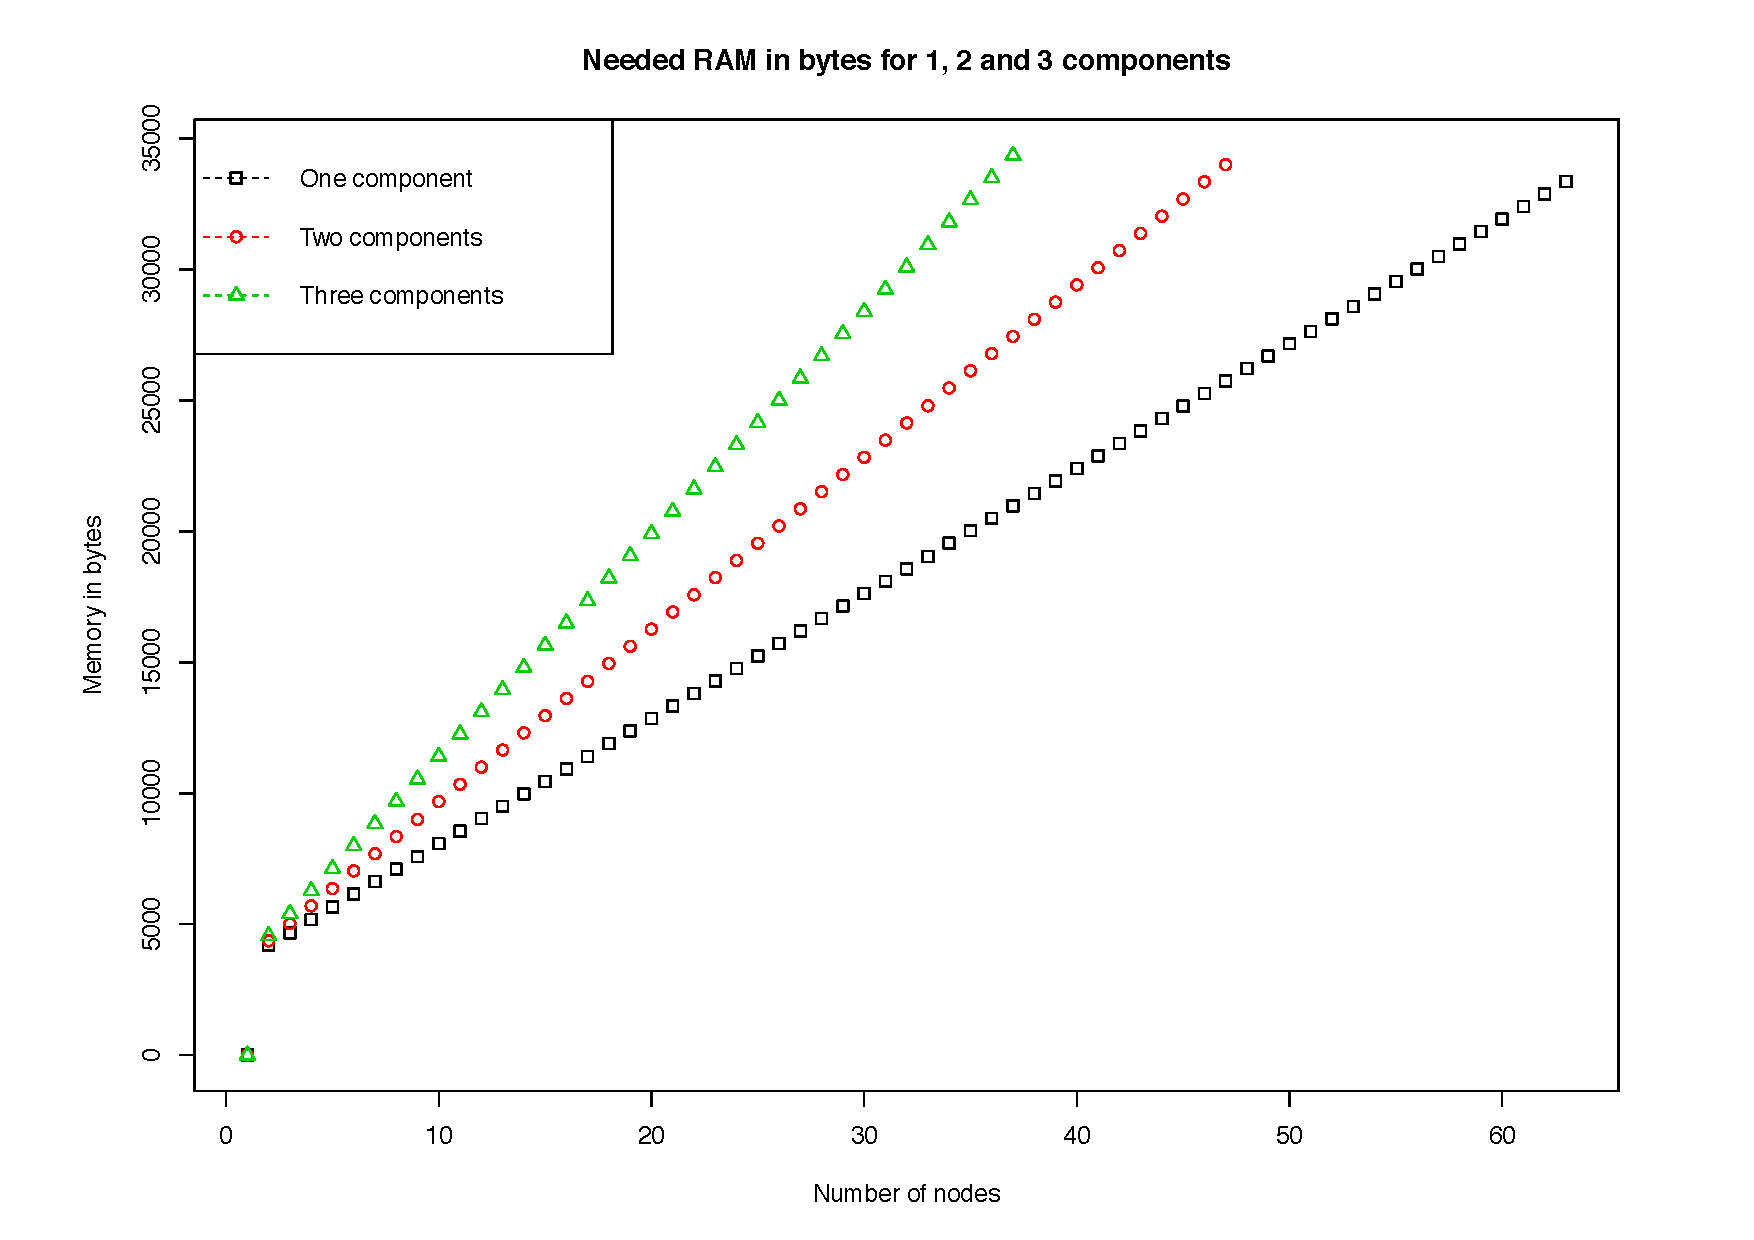
\includegraphics[width=1\columnwidth]{chapters/intra-node.images/memoryOverhead3NodesRemb.pdf}
	\caption{Memory overhead for 1, 2 and 3 \emph{Blink/COAP} components.} \label{fig:MemUsedBlinkComps}
\end{figure}


Figure \ref{fig:MemUsedBlinkComps} shows the memory usage for each model depending on its size.
These results show that our current implementation enables to scale the model up to 60 nodes with one component per node, and up to 37 nodes with three components per node. These numbers are encouraging, since some tens of nodes can enable a small IoT local network, such as home, small buildings, cars, factory chains, etc.


\section{Summary}
Our initial results show that the models@runtime implementation is feasible for IoT devices and there are enough resources to deploy several other functional software components.
Indeed, we can observe that our overheads are small enough to affect the overall operation of a node, while adding an abstract representation of the running system, in addition to reconfiguration and adaptation possibilities.
Since these results are promising, we highlighted that our middleware is able to represent a running application by abstracting it through a component model, without an important overhead, neither in memory nor in energy consumption.
The Contiki OS provides most of the functionalities that are mandatory for the good implementation of our models@runtime middleware.
As we described in this chapter, two crucial functionalities were not implemented on the IoT-Lab M3 platform: the File System and the ELF Loader.
Indeed, without these functionalities the adaptations generated by the model@runtime engine could not be executed.
Since the goal of our middleware is to deploy new modules by the means of an ELF file, these contributions are mandatory.
Naturally, easy storage and access for this file simplifies the task of loading, by leveraging the abstractions proposed by the Contiki File System.
Moreover, by adding the relocation and dynamic linking mechanisms to the M3 platform, real deployment of new features is now possible.

The added support for the two main functionalities needed by our middleware was crucial for the continuation of our research, since it allowed to conduct the evaluation on real nodes.
Without them, our experimentations would have stopped at the model level, without enacting the actual changes represented in the model at the system level.
The relevancy of our implementations was acknowledged by the FIT IoT-Lab maintainers, who accepted our pull-request\footnote{\url{https://github.com/iot-lab/contiki/pull/2}} including this technical contributions in their main fork of the Contiki repository.

In order to continue our research goals, we need to review our results and the tools already provided by our middleware.
Indeed, several challenges were raised with the results of our first model@runtime implementation.
%The first one, lies in the way that the model should be spread across the network.
%Since the same model must be present in all the nodes forming the network, we must investigate epidemic algorithms of distribution, such as Deluge \cite{hui2004dynamic}.
One of these challenges is about the creation of components and their distribution across the network.
Indeed, special attention should be put on this inter-node mechanism, since we have argued throughout this thesis that most of the energy consumption is due to radio communication, on battery powered wireless nodes.
Therefore, distributing software components on mesh topologies, which are less robust than typical computer networks, raise scientific questions about the best method to distribute them.
Thus, a distributed algorithm to download components taking into account the inter-node network topology and energy consumption should be proposed.
The next chapter will discuss how these components can be built, and how they can be distributed in an energy-efficient manner.

